\section{Results}
\label{sec:Results}
% Chaos
Plotting the probability of chaos against the competition parameter, we observe a clear maximum around $ \epsilon = 0 $. The likelihood of chaotic behaviour for neutral-on-average competition at the prey level is thus higher than for dominant inter or intraspecific competition. This result remains true for systems with a different number of species (figure \ref{fig:Contour}).

The overall likelihood of chaos increases with the size of the food web. This effect should not be surprising: the more dimensions the phase space has, the easier is to fulfill the requirements of the complex geometry of a chaotic attractor \citep{Strogatz1994}. Even in those higher dimensional cases, there is still a clear maximum at neutral-on-average competition. Another local maximum was observed for low values of $ \epsilon $, meaning that weak competitive coupling also promotes chaos in our model.

\begin{figure}
	\begin{center}
		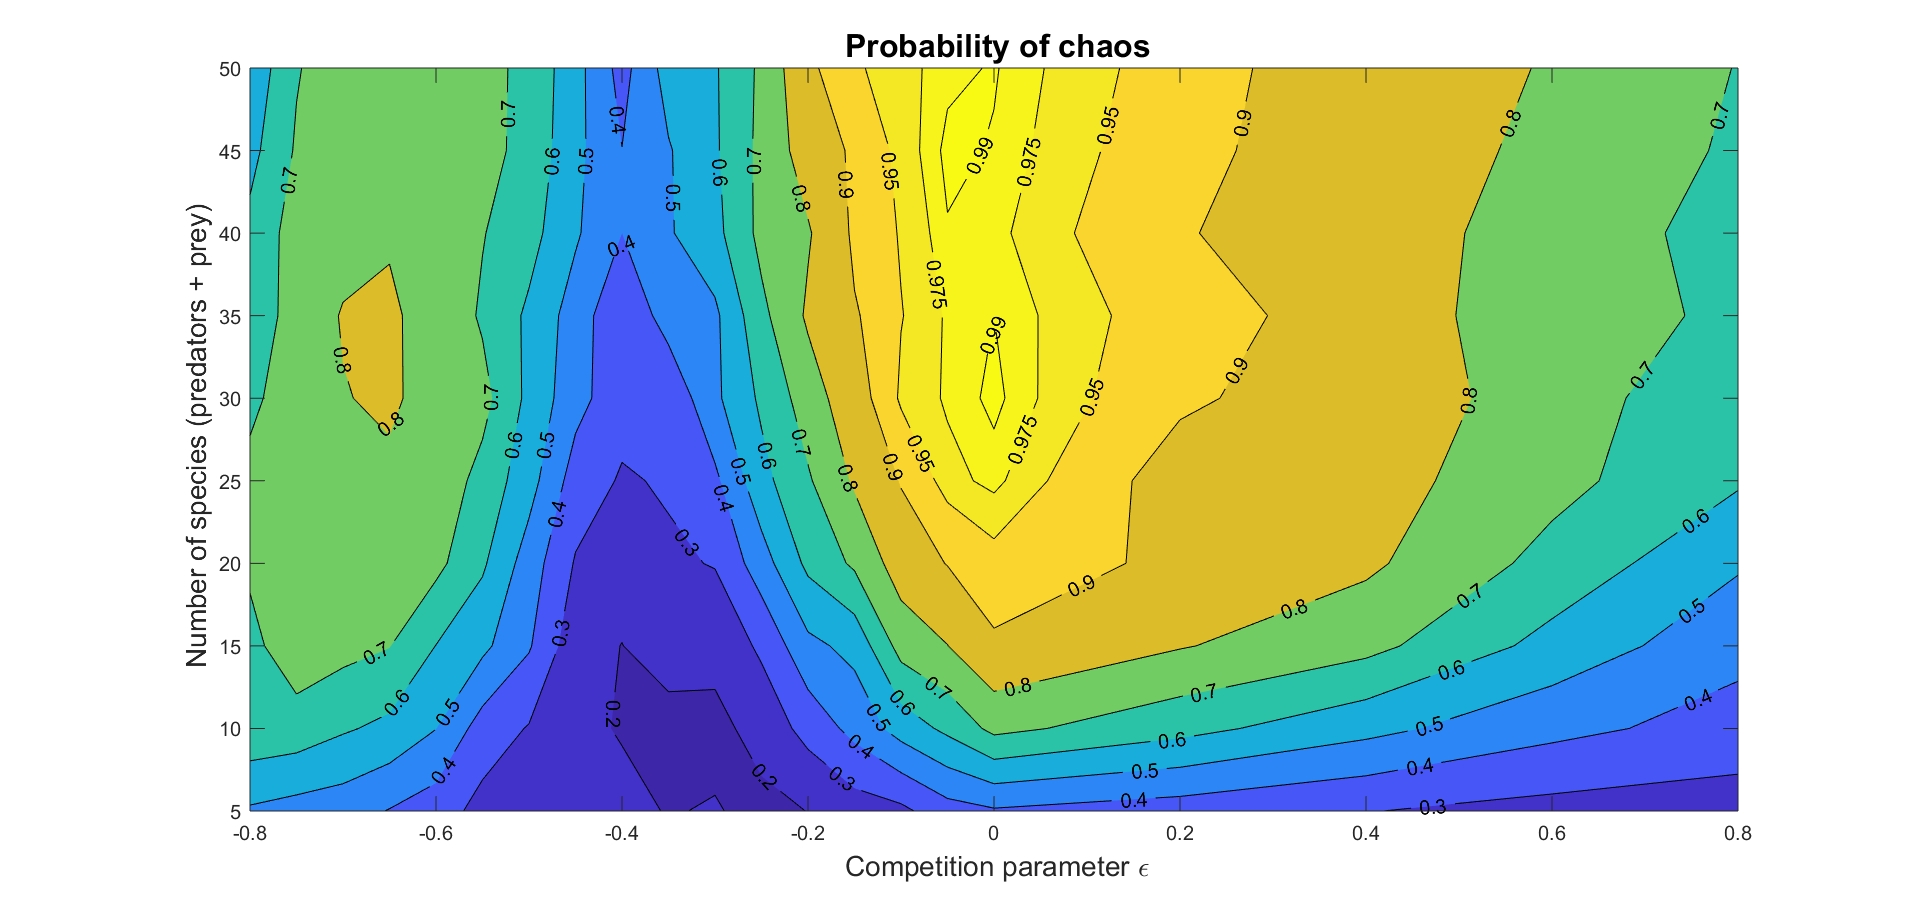
\includegraphics[width=1\columnwidth]{contour.png}
	\end{center}
	\caption{Contour map showing the probability of chaos for various competition parameters (horizontal axis) and number of species (vertical axis). The consumers' population is fixed as $ 2/3 $ of the prey's population. Notice that chaotic attractors appear more easily (i.e., for smaller systems) the closer is the competition to neutral (i.e., $ \epsilon = 0 $).}
	\label{fig:Contour}
\end{figure}

% Biodiversity
Our biodiversity measures (see figure \ref{fig:Biodiversity}) illustrate two additional effects: chaos clearly tends to increase biodiversity in our model and overall biodiversity is very close to its maximum around neutral-on-average situation.

\begin{figure}
	\begin{center}
		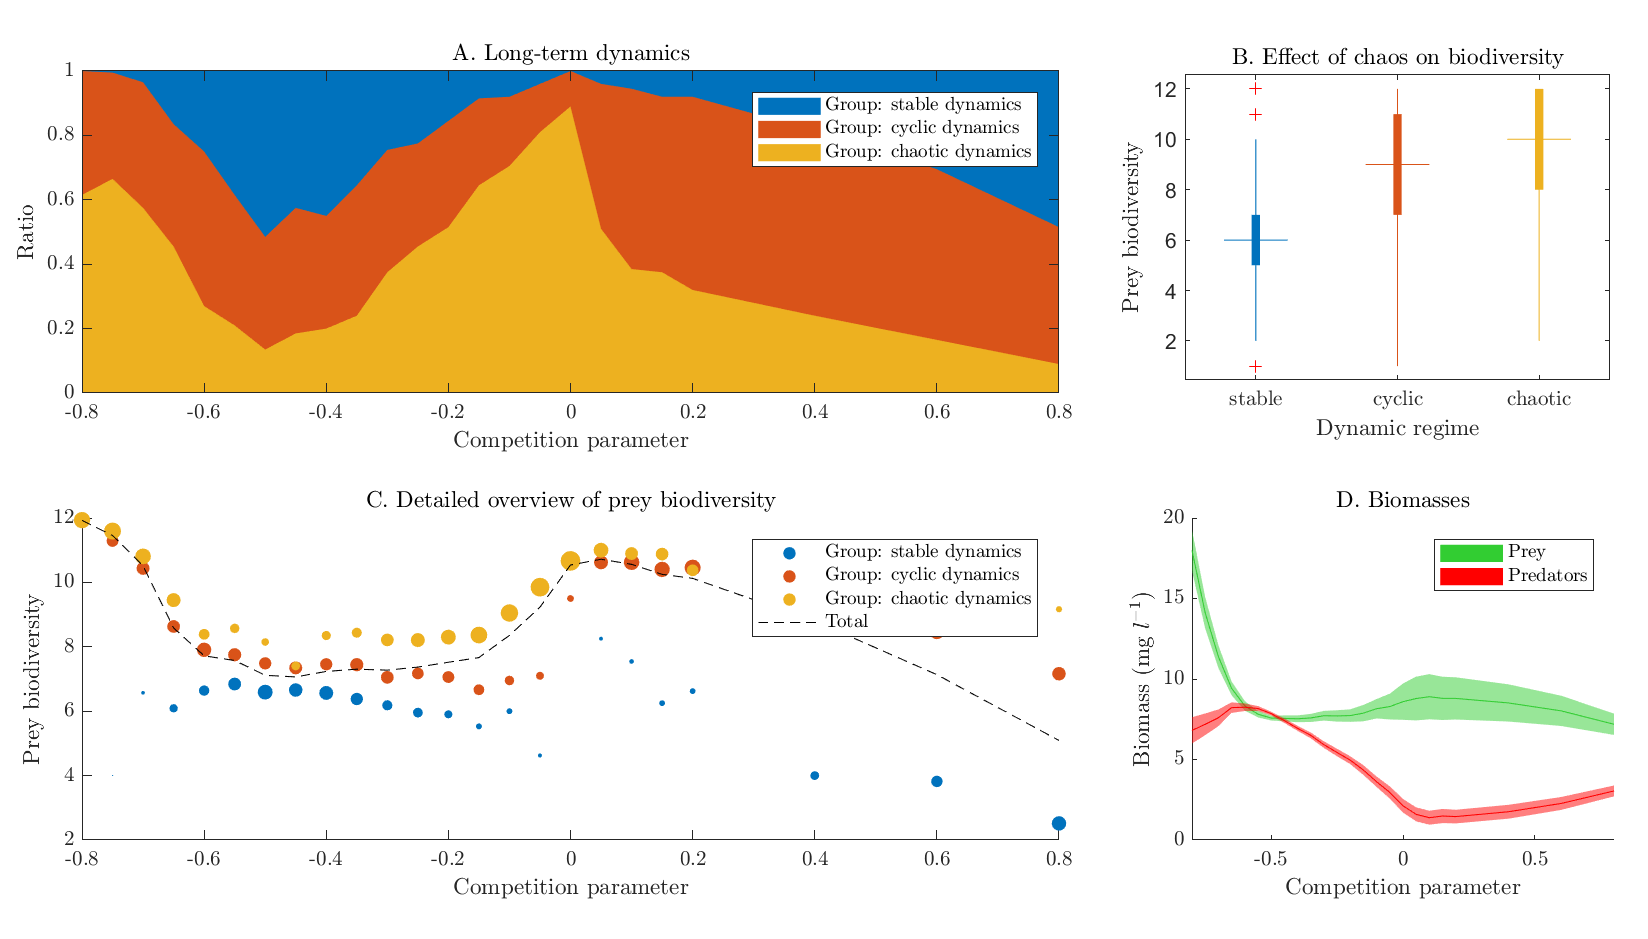
\includegraphics[width=1\columnwidth]{best.png}
	\end{center}
	\caption{Results for a food web with $8$ predator and $12$ prey species. Food webs of different sizes show similar results (see \ref{subsec:ExtraFigures} in Online Appendix). For each value of the competition parameter, $\numReps$ randomly drawn ecosystems were simulated and classified as regular, cyclic or chaotic. Additionally, the number of non-extinct prey species after a stabilization run was registered. \textbf{Panel A} Ratio of each dynamic regime vs. competition parameter. \textbf{Panel B} Biodiversity vs. asymptotic regime. Box and whisker plot of the average number of non-extinct prey species grouped by asymptotic regime. \textbf{Panel C} Average prey biodiversity vs. competition parameter. The dashed line shows the average number of non-extinct prey species grouped by competition parameter. The colored circles represent the average prey biodiversity of the simulations, additionally grouped by dynamical regime (stable, cyclic and chaotic). The relative size of the circles represents the ratio of simulations that led to regular or chaotic dynamics. \textbf{Panel D} Average biomasses grouped by trophic level vs. competition parameter. The width represents standard deviation.}
	\label{fig:Biodiversity}
\end{figure}